
\section{Evaluation}
\label{sec:eval}

In this section, we will compare the performance of original LibFuzzer, our LibFuzzer and AFL. We use fuzzer-test-suite\cite{fuzzer-test-suite}, a set of tests for fuzzing engines provided by Google, as the test cases. In order to support our LibFuzzer, we modify the \texttt{target.cc} in some test cases. Take \texttt{c-ares-CVE-2016-5180} for example, we modified the \texttt{extern "C" int LLVMFuzzerTestOneInput(const uint8\_t *Data, size\_t Size)} function declaration to \texttt{int main()}. And use \texttt{read} function to read input data, the size is the length of input data. Check out more detail of patching fuzzer-test-suite in wiki page of our repository. The following specification is our machine information and all experiments were performed on it.

\begin{lstlisting}
virtual private server on Google Cloud Platform
n1-standard-1 (one vCPU, 3.75 GB RAM)
\end{lstlisting}

\subsection{Compared with original LibFuzzer}

We choose some CVE test cases in fuzzer-test-suite, including \texttt{CVE-2016-5180}, \texttt{CVE-2015-8317} and \texttt{HeartBleed (CVE-2014-0160)}, to evaluate the performance of our LibFuzzer. These are the output of running test cases by our LibFuzzer and do it 10 times to calculate the average time.

\begin{enumerate}
    \item [1.] \texttt{CVE-2016-5180}
\end{enumerate}

This is a 1-byte-write-heap-buffer-overflow in c-ares. This bug was one of out a chain of two bugs that made a ChromeOS exploit possible: code execution in guest mode across reboots.

\begin{lstlisting}
#0      READ units: 1
#2      INITED cov: 4 ft: 20 corp: 1/1b exec/s: 2 rss: 25Mb
#3      NEW    cov: 4 ft: 39 corp: 2/3b exec/s: 3 rss: 25Mb L: 2/2 MS: 1 CopyPart-
#4      pulse  cov: 4 ft: 59 corp: 2/3b exec/s: 2 rss: 25Mb
#4      NEW    cov: 4 ft: 59 corp: 3/5b exec/s: 2 rss: 25Mb L: 2/2 MS: 2 CopyPart-ShuffleBytes-
Error status : 139
Signal : Segmentation fault
\end{lstlisting}

And we can find the 1-byte-write-heap-buffer-overflow by our LibFuzzer within 3 seconds.

\begin{enumerate}
    \item [2.] \texttt{CVE-2015-8317}
\end{enumerate}

This is a 1-byte-read-heap-buffer-overflow and a memory leak in libxml2.

\begin{lstlisting}
#0      READ units: 1
Error status : 139
Signal : Segmentation fault
\end{lstlisting}

Using our LibFuzzer can find the 1-byte-read-heap-buffer-overflow and a memory leak within 120 seconds.

\begin{enumerate}
    \item [3.] \texttt{HeartBleed (CVE-2014-0160)}
\end{enumerate}

This is a multi-byte-read-heap-buffer-overflow in openssl.

\begin{lstlisting}
#0      READ units: 1
...
Error status : 134
Signal : Aborted
\end{lstlisting}

In this test case, we cannot find the multi-byte-read-heap-buffer-overflow because this is a network service and there are a few asserts cannot pass by running program in local. As a result, we only got an aborted signal not segmentation fault.

Compared with original LibFuzzer and plot the chart.

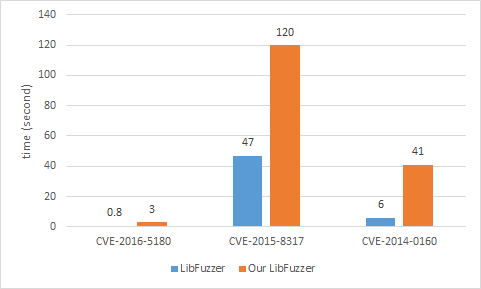
\includegraphics[width=\linewidth]{eval1.png}

As we can see, because the implementaion of our LibFuzzer, the IO speed and analysis take a lot of time. And the preformance is slower than original LibFuzzer. But compared the time of original LibFuzzer and our LibFuzzer took, we still can find the bugs efficiently in these test cases.

\subsection{Compared with AFL}

According to the section of binary-only instrumentation in the technical whitepaper for afl-fuzz, we know the overhead of the QEMU mode is roughly 2-5x. So we try to compare with the overhead, the time of linking IO and analyzing the output, between AFL and our LibFuzzer. And the following chart is the overhead of the test cases we ran before.

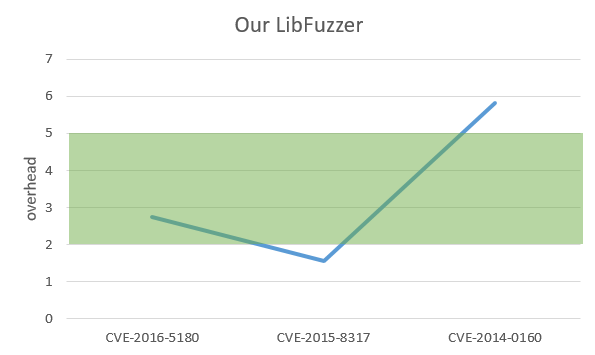
\includegraphics[width=\linewidth]{eval2.png}

The green area is the overhead of the QEMU mode and the bule line is our LibFuzzer overhead. We can see the result is close to the QEMU mode and therefore it maybe cost that much time to do analyze and link IO for supporting binary only mode.

